\chapter{Supplemental Material for Chapter \ref{chap:Ciona intestinalis gastrulation}}

%%%%%%%%%%%%%%%%%%%%%%%%%%%%%%%%%%%%%%%%%%%%%%%%%%%%%%%%%%%%%%%%%%%%%%%%%%%%%%%%
\section{Supplementary Figures}
%%%%%%%%%%%%%%%%%%%%%%%%%%%%%%%%%%%%%%%%%%%%%%%%%%%%%%%%%%%%%%%%%%%%%%%%%%%%%%%%

%%%%%%%%%%%% Figure S1 is large, so we need to split things! 
\begin{figure}[h]
    \centering
    \caption[Quality control of the \textit{Ciona} single-cell gastrulation atlas]{\textbf{A.} Distribution of number of gene counts per cell across all time points (4.5 hours post fertilization (hpf), 5.5 hpf, and 6.5 hpf) and all biological replicates. \textbf{B.} Scatterplot of the number of gene counts per cell versus the number of genes per cell across the entire gastrulation atlas. \textbf{C-D.} Histograms of the number of gene counts per cell (C) and the number of genes per cell (D) across the entire gastrulation atlas. \textbf{E-F.} UMAP visualizations of the single-cell gastrulation atlas colored by time point (E) and by Leiden clustering (F). (\textit{Continued on next page.})}
    \label{fig:quality control single cell atlas}
\end{figure}

\addtocounter{figure}{-1}

\captionsetup[figure]{list=no}
\begin{figure}[p]
    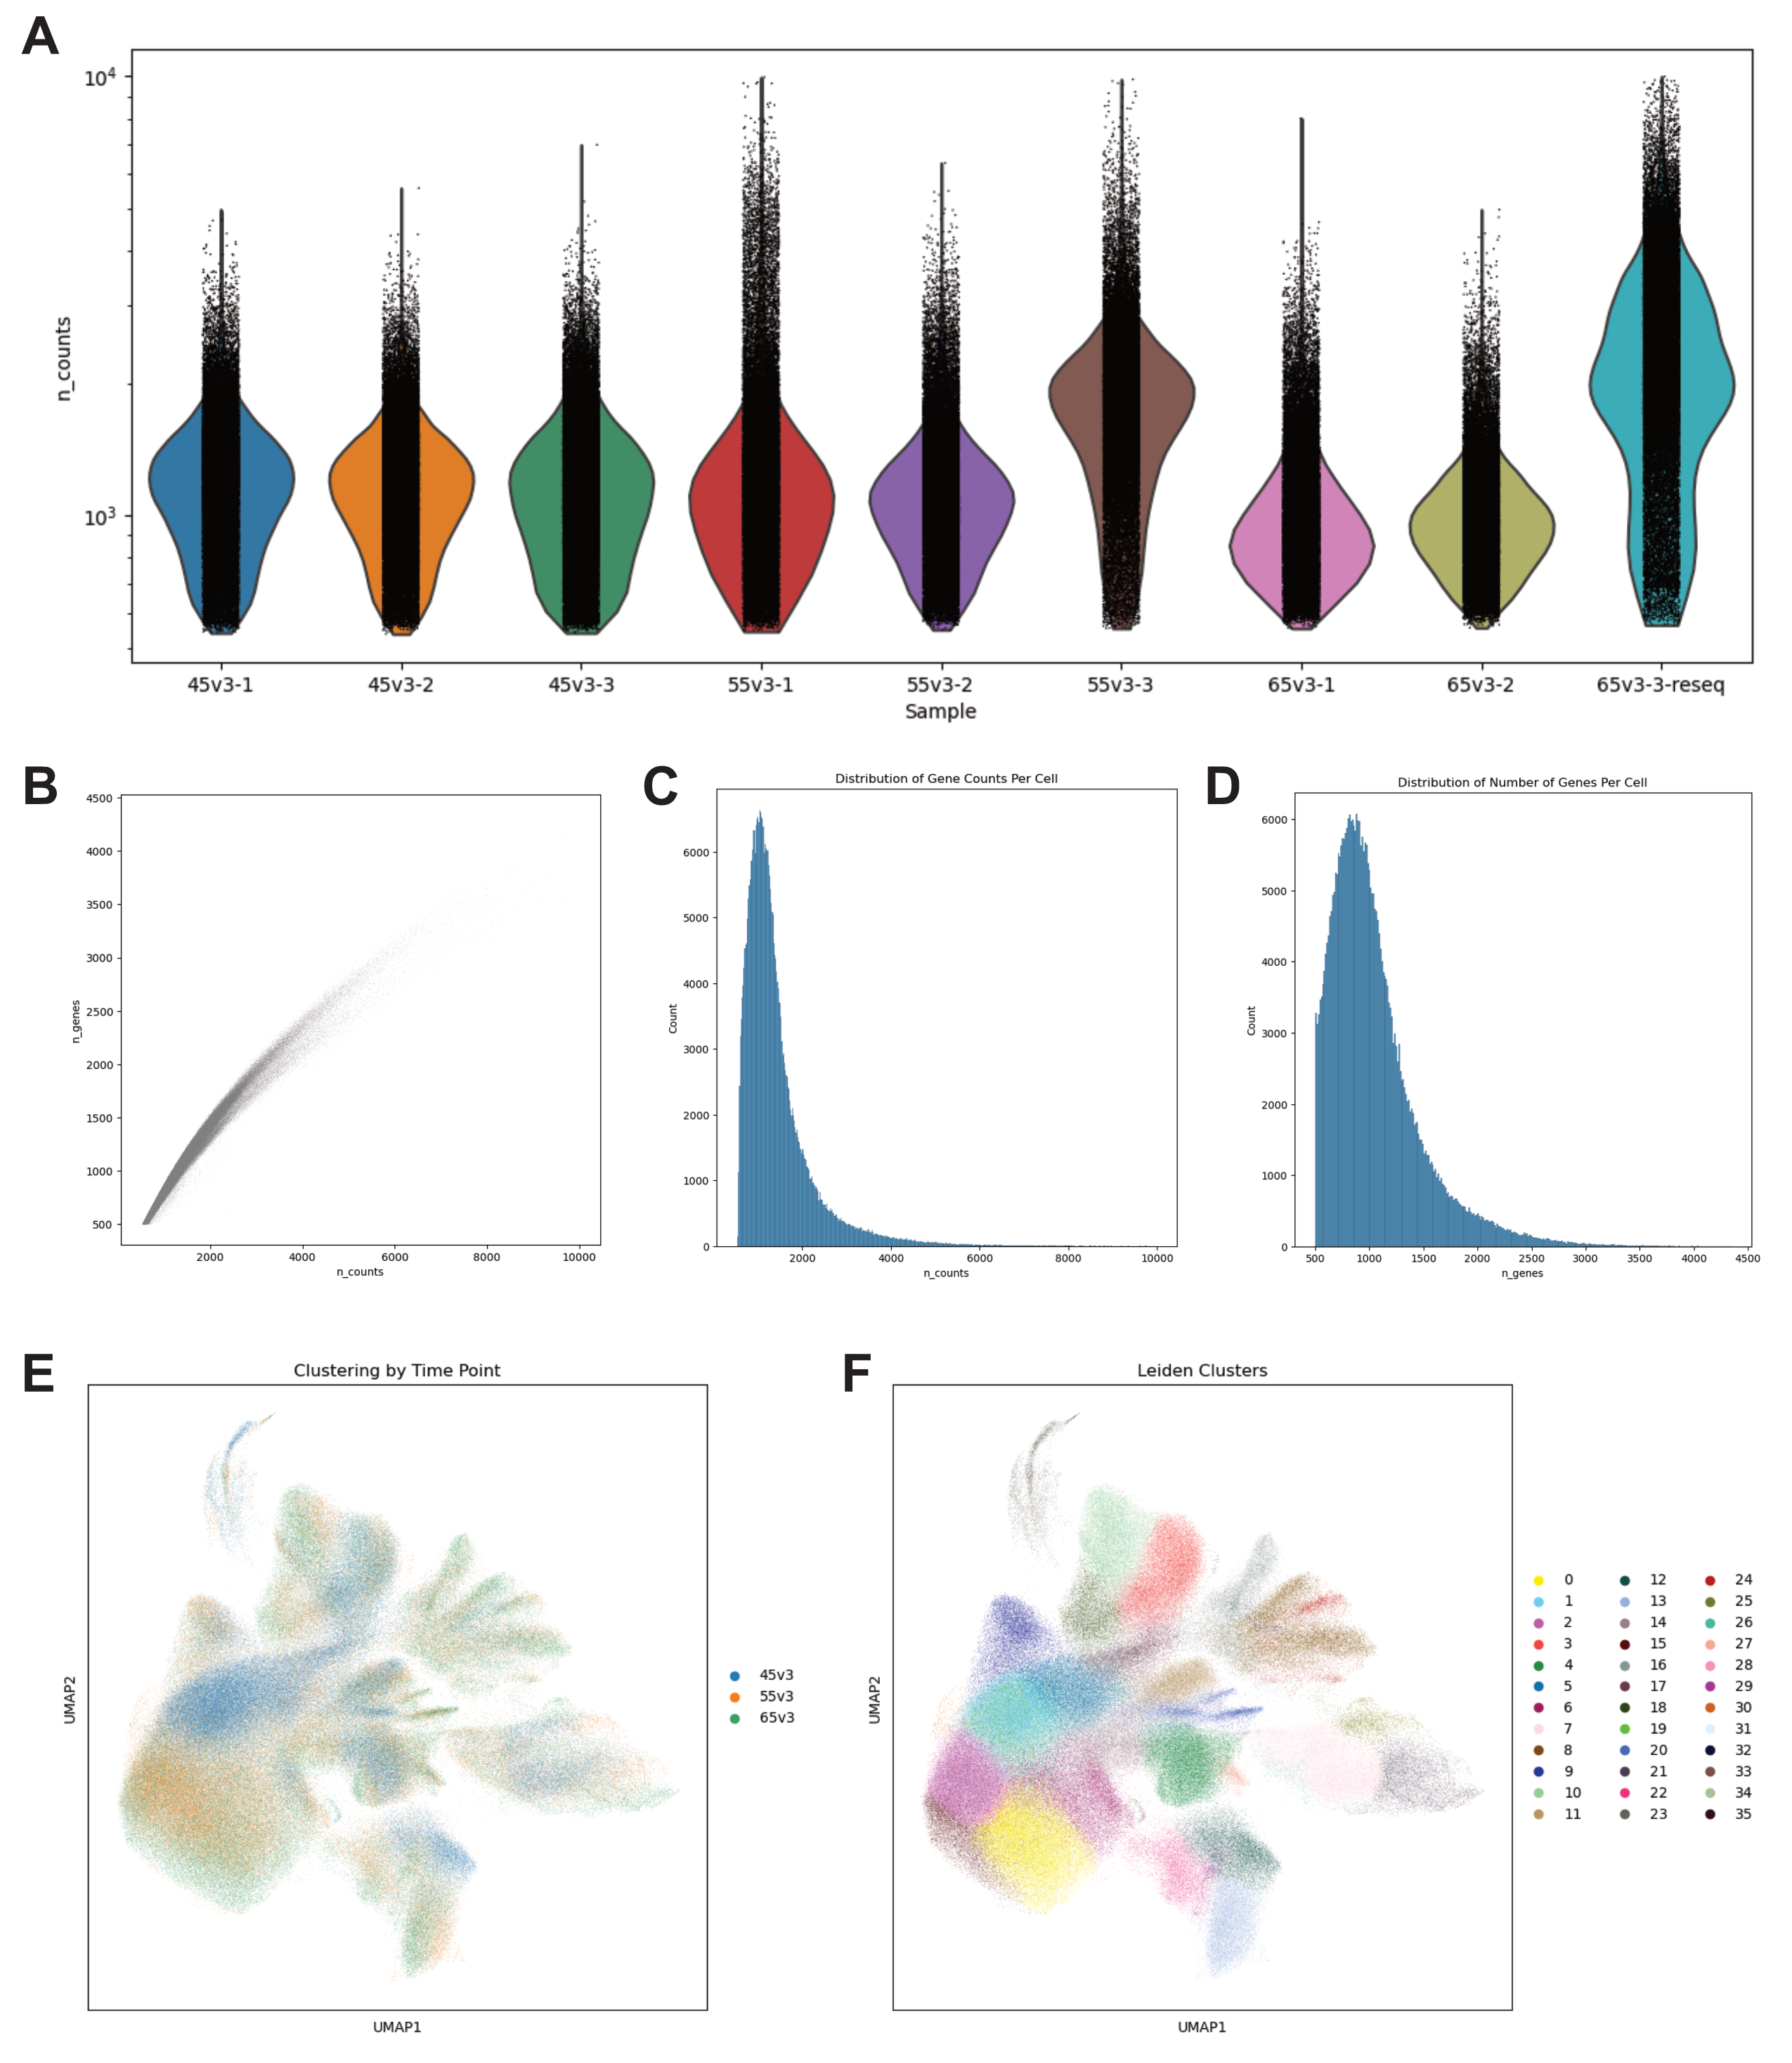
\includegraphics[scale=.73]{4_figures-and-files/FigS1_Quality-Control-Metrics.png}
    \caption{(\textit{Continued from previous page.})}
\end{figure}
\captionsetup[figure]{list=yes}
%%%%%%%%%%%%